\documentclass{beamer}
 
\usepackage[utf8]{inputenc}


\usetheme{Madrid}
\usecolortheme{default}
\usepackage{caption}
\usepackage{subcaption}
\usepackage{hhline}
\usepackage{graphicx}
\usepackage{physics}
\usepackage{amsmath}
\usepackage{amsfonts}
\usepackage{esint}
\usepackage{bbold}
\usepackage{mathtools}
\usepackage{dsfont}
\usepackage{amsthm}
\usepackage{bbm}
\usepackage{amssymb}
\theoremstyle{definition}
\newtheorem{defn}{Definition}[section]
\newtheorem{prop}{Properties}[section]
\newtheorem{rmk}{Remark}[section]
\newtheorem{exmp}{Example}[section]
\newtheorem{prob}{Problem}[section]
\newtheorem{proposition}{Proposition}
\newtheorem{thm}{Theorem}[section]
\newtheorem*{prob*}{Problem}
\newtheorem*{sln*}{Solution}
\usepackage{empheq}
\usepackage{tensor}

\newcommand{\lag}{\mathcal{L}}
\newcommand{\pOne}{\text{5p}_\text{1/2}}
\newcommand{\pThree}{\text{5p}_\text{3/2}}
\newcommand{\potassium}{^\text{39}\text{K}}
\newcommand{\R}{\mathbb{R}}
\newcommand{\lp}{\left(}
\newcommand{\rp}{\right)}
\newcommand{\lb}{\left[}
\newcommand{\rb}{\right]}
\newcommand{\lc}{\left\{}
\newcommand{\rc}{\right\}}
\newcommand{\p}{\partial}
\newcommand{\f}[2]{\frac{#1}{#2}}
\newcommand{\Vol}{\operatorname{Vol}}
\newcommand{\iprod}{\mathbin{\lrcorner}}
\newcommand{\al}{\alpha}
\newcommand{\be}{\beta}
\newcommand{\FT}{\mathcal{F}}
\newcommand{\LT}{\mathcal{L}}
\usepackage{hyperref}
\usepackage{tensor}
\usepackage{xcolor}
\hypersetup{
	colorlinks,
	linkcolor={black!50!black},
	citecolor={blue!50!black},
	urlcolor={blue!80!black}
}

% 3j symbol
\newcommand{\tj}[6]{ \begin{pmatrix}
		#1 & #2 & #3 \\
		#4 & #5 & #6 
\end{pmatrix}}
% 6j symbol
\newcommand{\Gj}[6]{ \begin{Bmatrix}
		#1 & #2 & #3 \\
		#4 & #5 & #6 
\end{Bmatrix}}



 
 
%Information to be included in the title page:
\title[\textcolor{white}{MOT-based Lifetime Measurements...}]
{
	MOT-based Lifetime Measurements of Potassium-39 $\text{5p}_\text{1/2}$ and $\text{5p}_\text{3/2}$ states
}



\author[Bui] % (optional)
{Huan Q. Bui \\
	$\,$ \\
	Advisor: Professor Charles Conover}

\institute[Colby College] % (optional)
{
}
\date{CLAS, April 28, 2021}
 
%\logo{
\includegraphics[height=0.3cm]{colby.png}}
 
\begin{document}
 
\frame{\titlepage}



%%%%%%%%%%%%%%%%%%%%%%%%%%%%%%%%%%%%%%%%%%%%%%%%%%%%%%%%%%%%%%%%%%%%%%%%%

 
%\begin{frame}
%\frametitle{Layout}
%\tableofcontents
%\end{frame}

%%%%%%%%%%%%%%%%%%%%%%%%%%%%%%%%%%%%%%%%%%%%%%%%%%%%%%%%%%%%%%%%%%%%%%%%%



\begin{frame}
\frametitle{Why lifetime measurements?}


\begin{equation*}
\frac{1}{\tau_{fi}} = \frac{4\alpha \omega_0^3}{3c^2}\abs{ \bra{f} e \mathbf{r} \ket{i}}^2
\end{equation*}


$\,$\\


\begin{itemize}
	\item Provide empirical data/constants
	\item Confidence in matrix element calculations for understanding fundamental physics (e.g. parity violation)
\end{itemize}


\end{frame}






\begin{frame}
\frametitle{Idea}
Excite the \textcolor{blue}{\textbf{MOT}} by a (short) 405 nm pulse, and observe fluorescence.
\begin{figure}[!htb]
	\vspace{-10pt}
	\centering
	\begin{subfigure}{0.55\textwidth}
	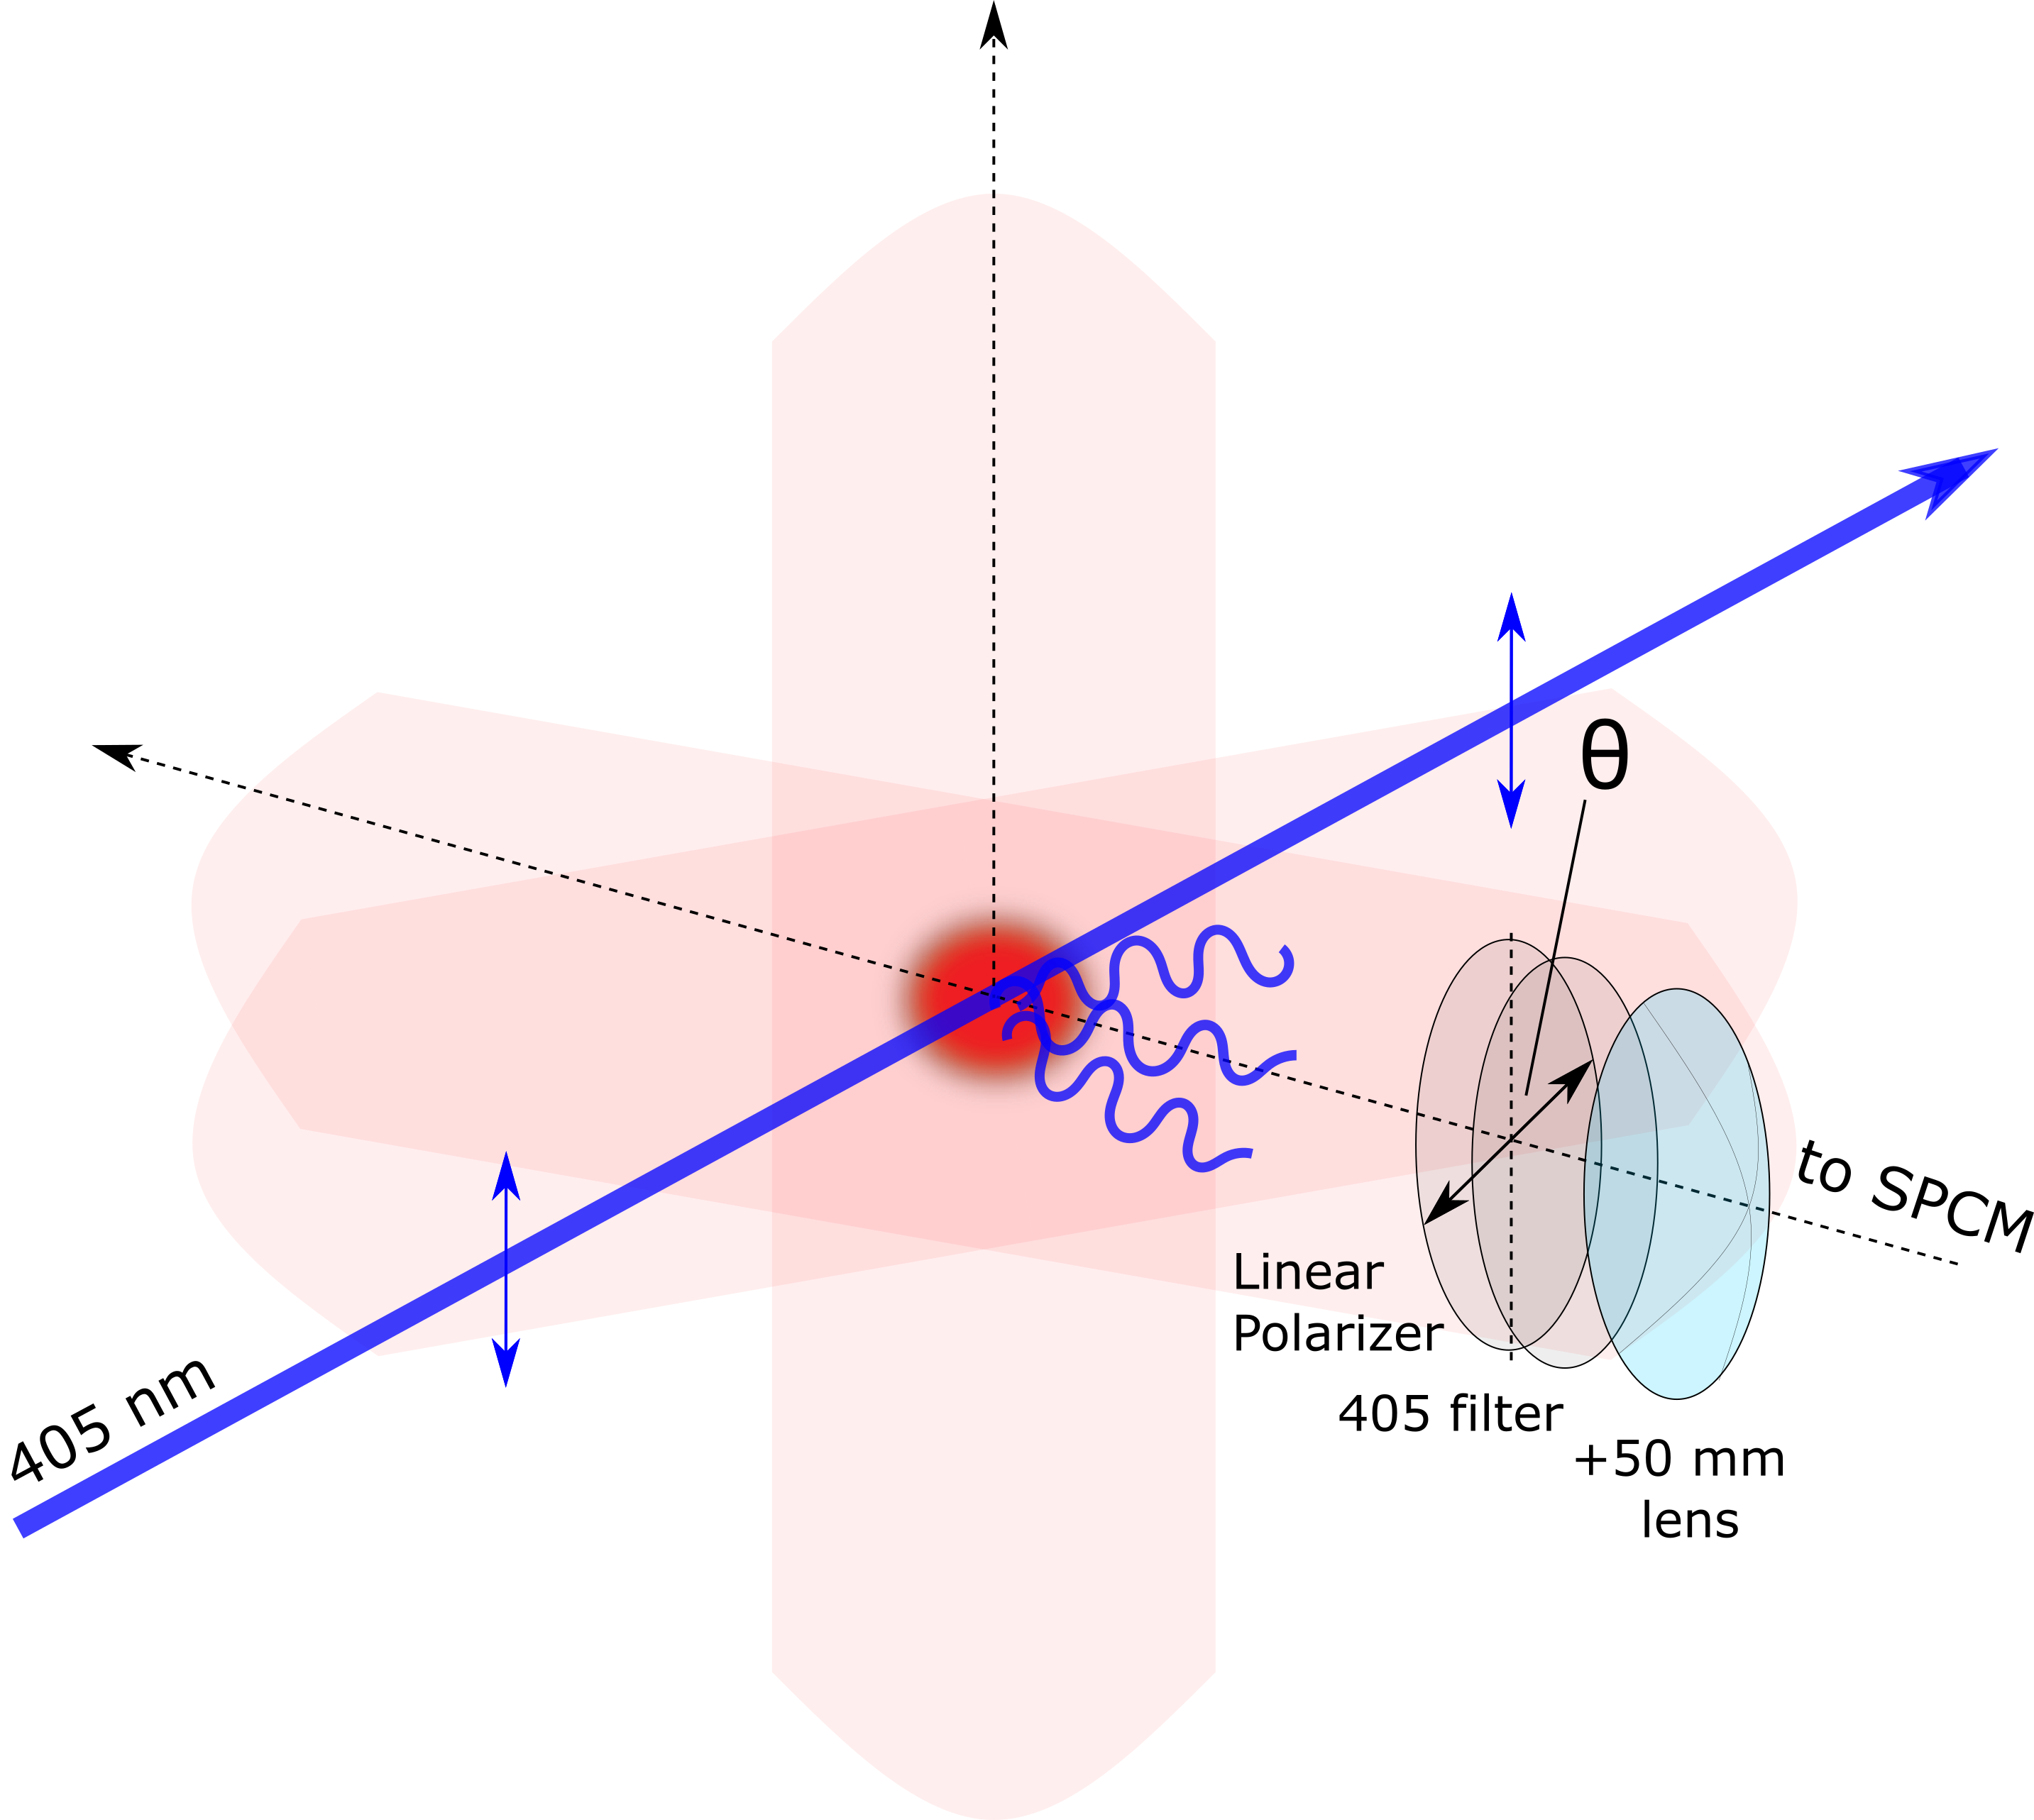
\includegraphics[width=0.8\textwidth]{experimental_geometry}
	\end{subfigure}
	\begin{subfigure}{0.4\textwidth}
	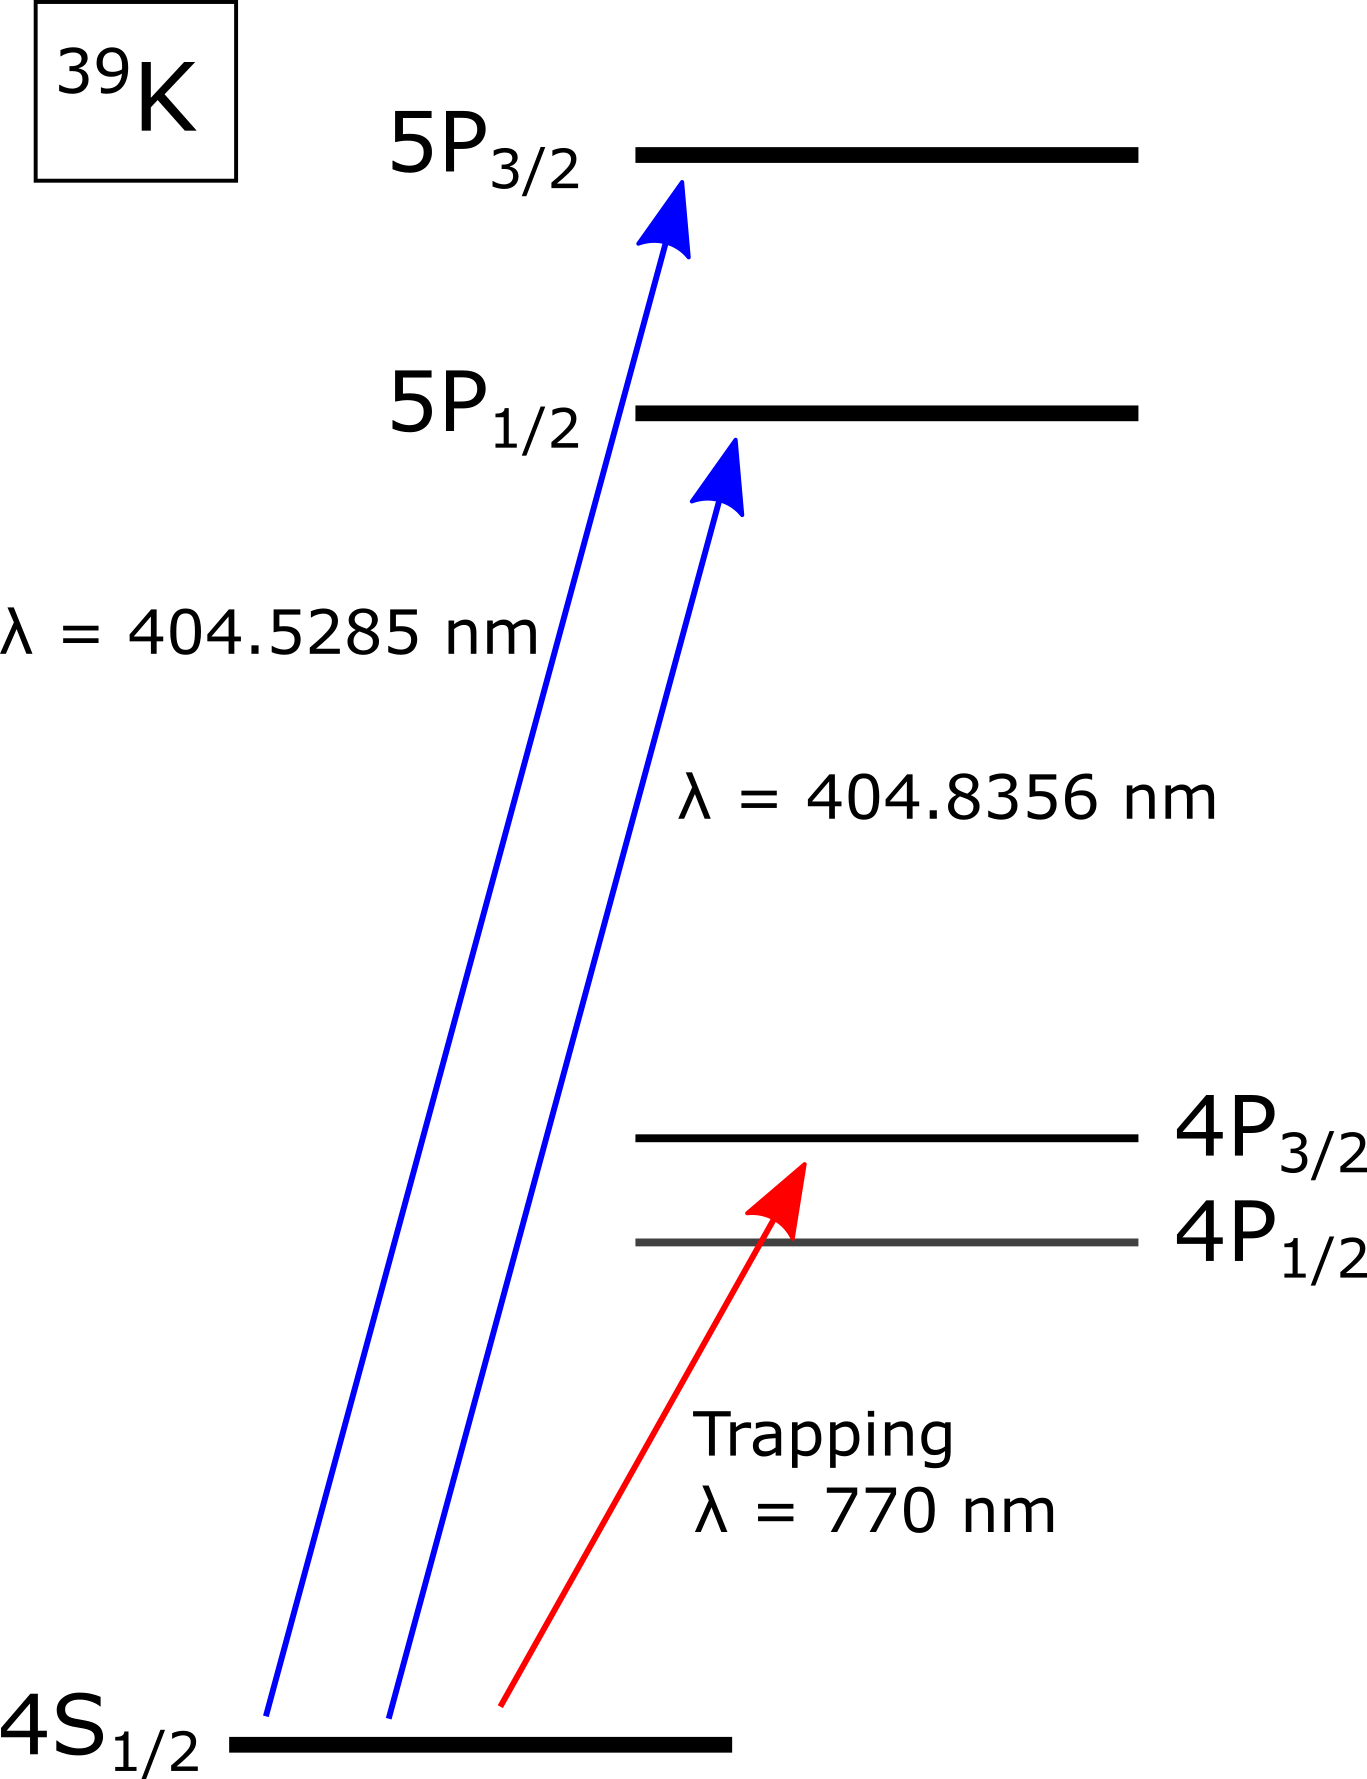
\includegraphics[width=0.7\textwidth]{energy_levels.png}
	\end{subfigure}
\end{figure}

Pulse 405 nm source at 250 kHz.\\
Cloud diameter $\sim$ 1 mm. T $\sim$ 1 mK. N $\sim$ 10$^\text{6}$ atoms.

\end{frame}


\begin{frame}
\frametitle{Idea}
Fluorescence should be an exponential decay. 

\begin{figure}[!htb]
	\vspace{-10pt}
	\centering
	\begin{subfigure}{0.55\textwidth}
		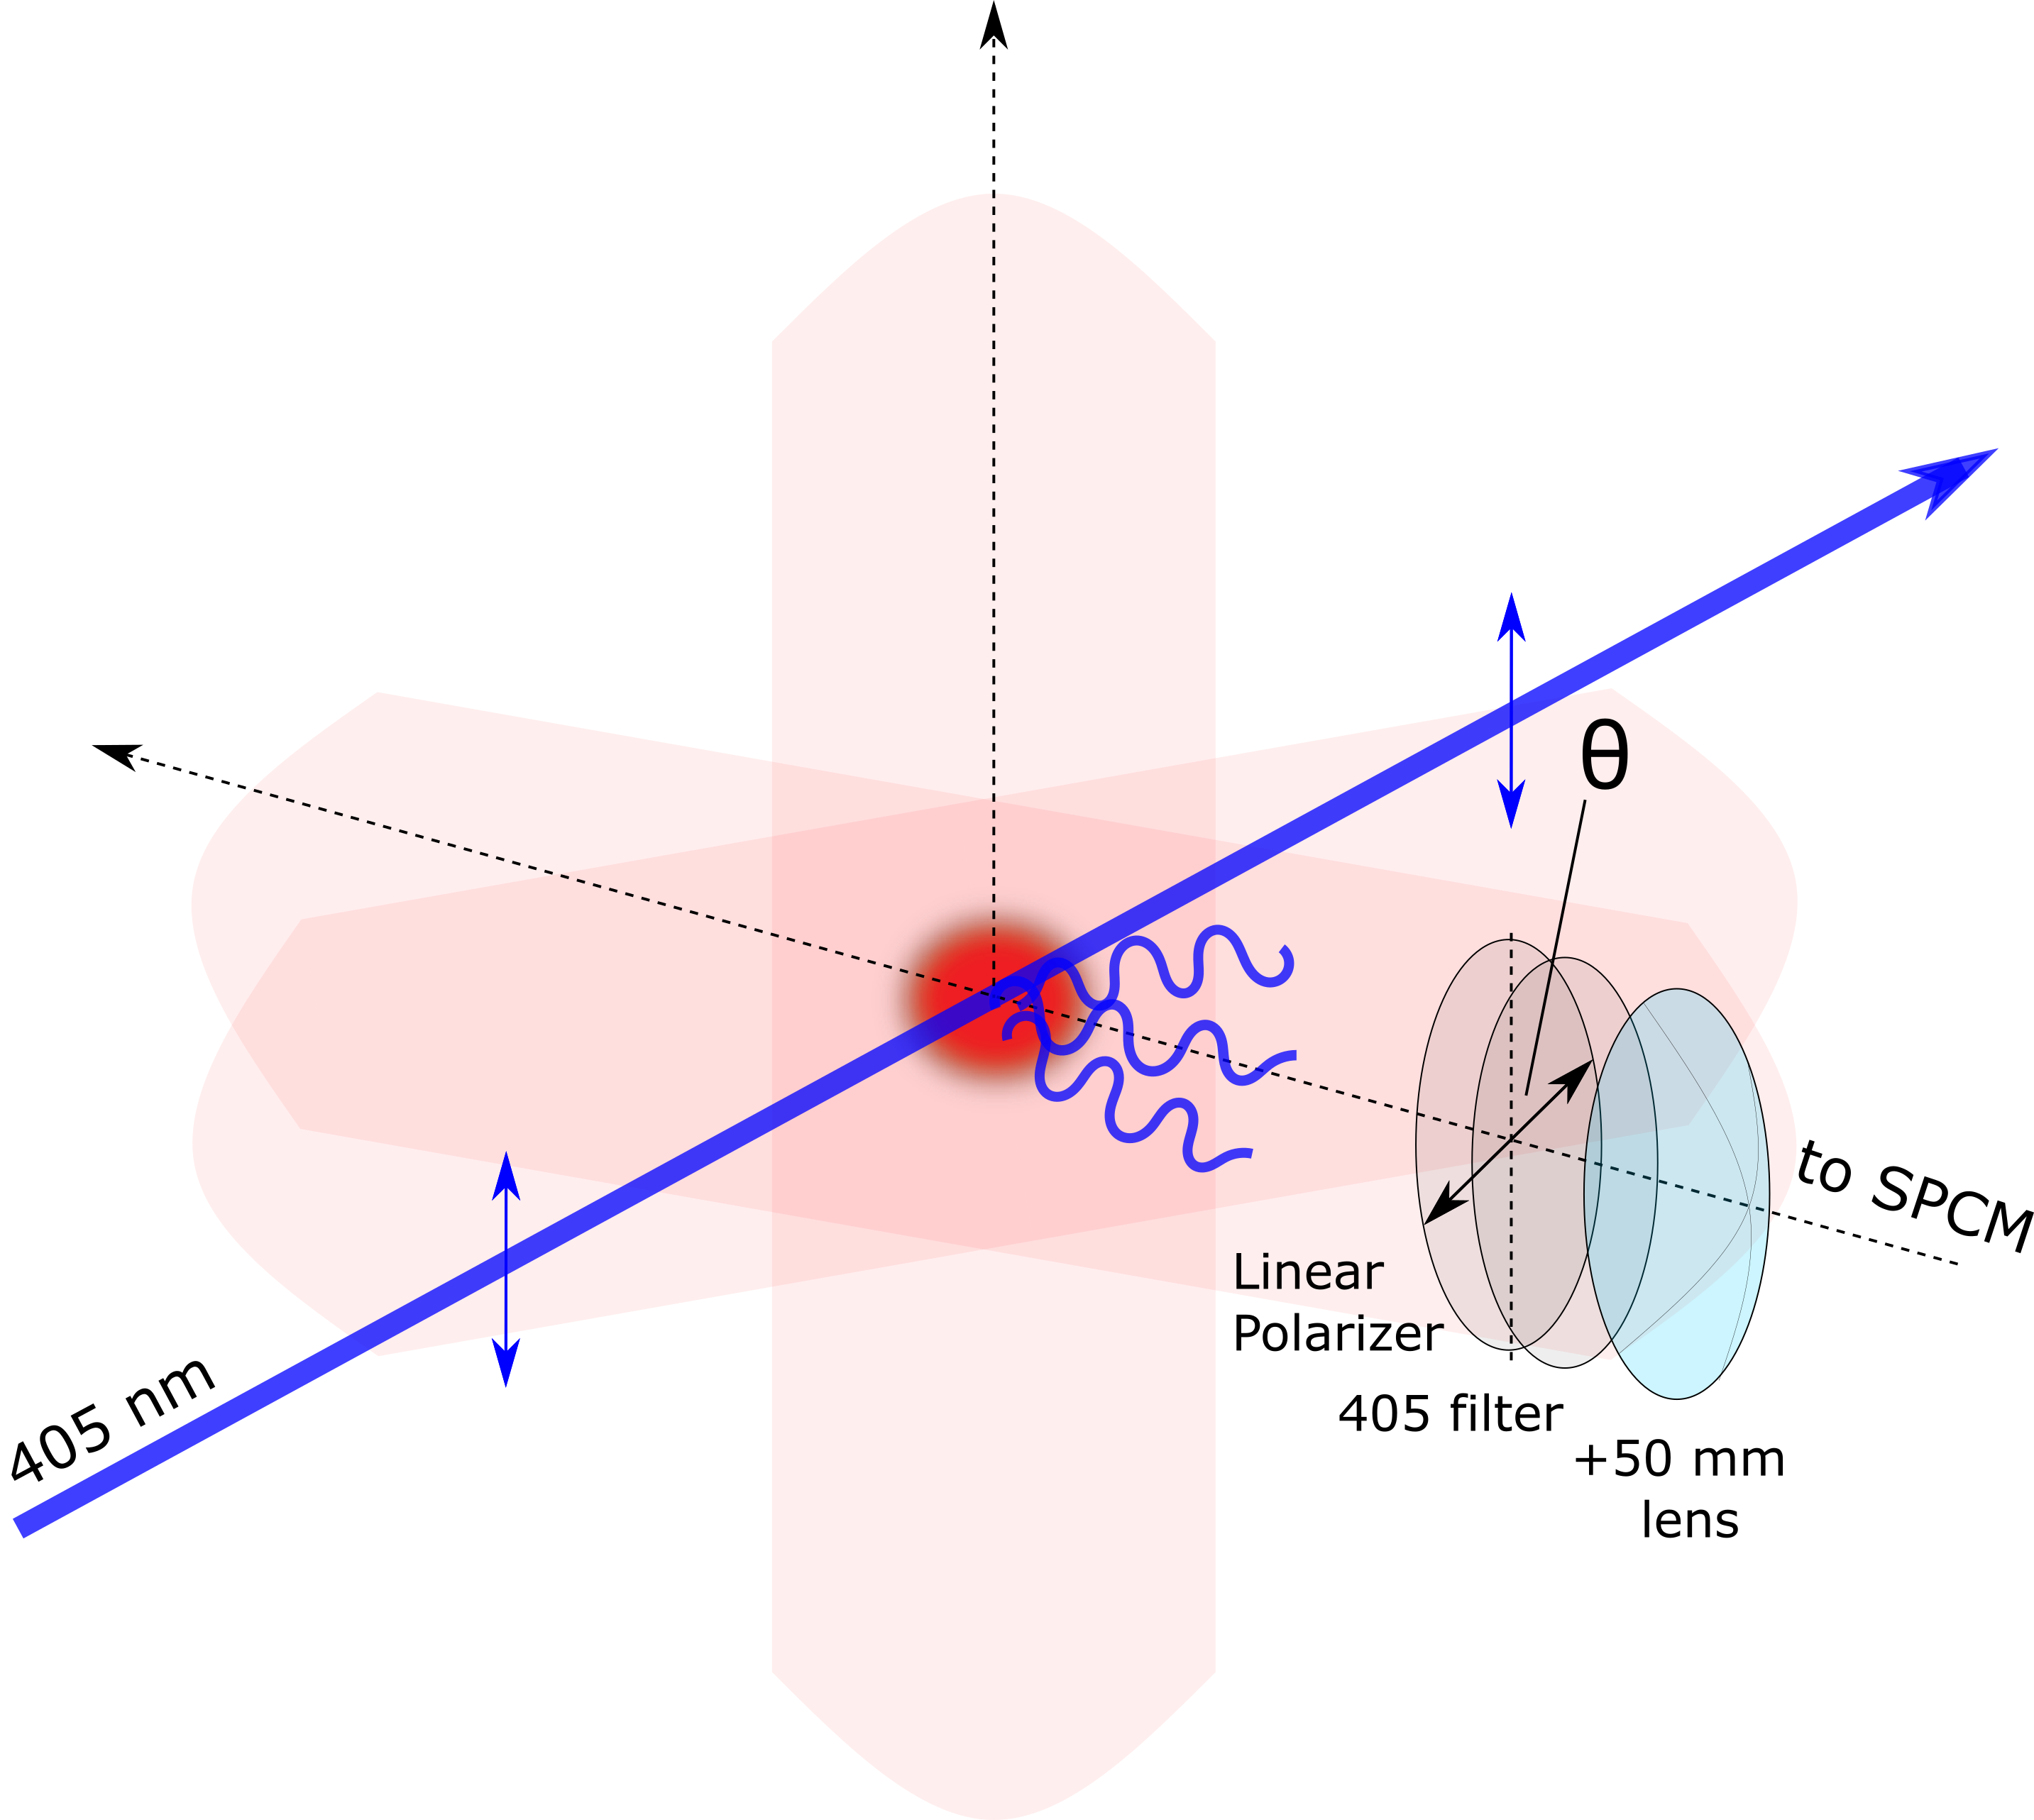
\includegraphics[width=\textwidth]{experimental_geometry}
	\end{subfigure}
	\begin{subfigure}{0.4\textwidth}
		\includegraphics[width=\textwidth]{p12_70ns_pol.eps}
	\end{subfigure}
\end{figure}

Data fitted with $N = Bkg + A\exp[-(t-t_0)/\tau]$. Residual is normalized. 

\end{frame}





\begin{frame}
\frametitle{Idea}
Fluorescence should be an exponential decay. 
\textcolor{purple}{\textbf{Or should it?}}

\begin{figure}[!htb]
	\vspace{-10pt}
	\centering
	\begin{subfigure}{0.55\textwidth}
		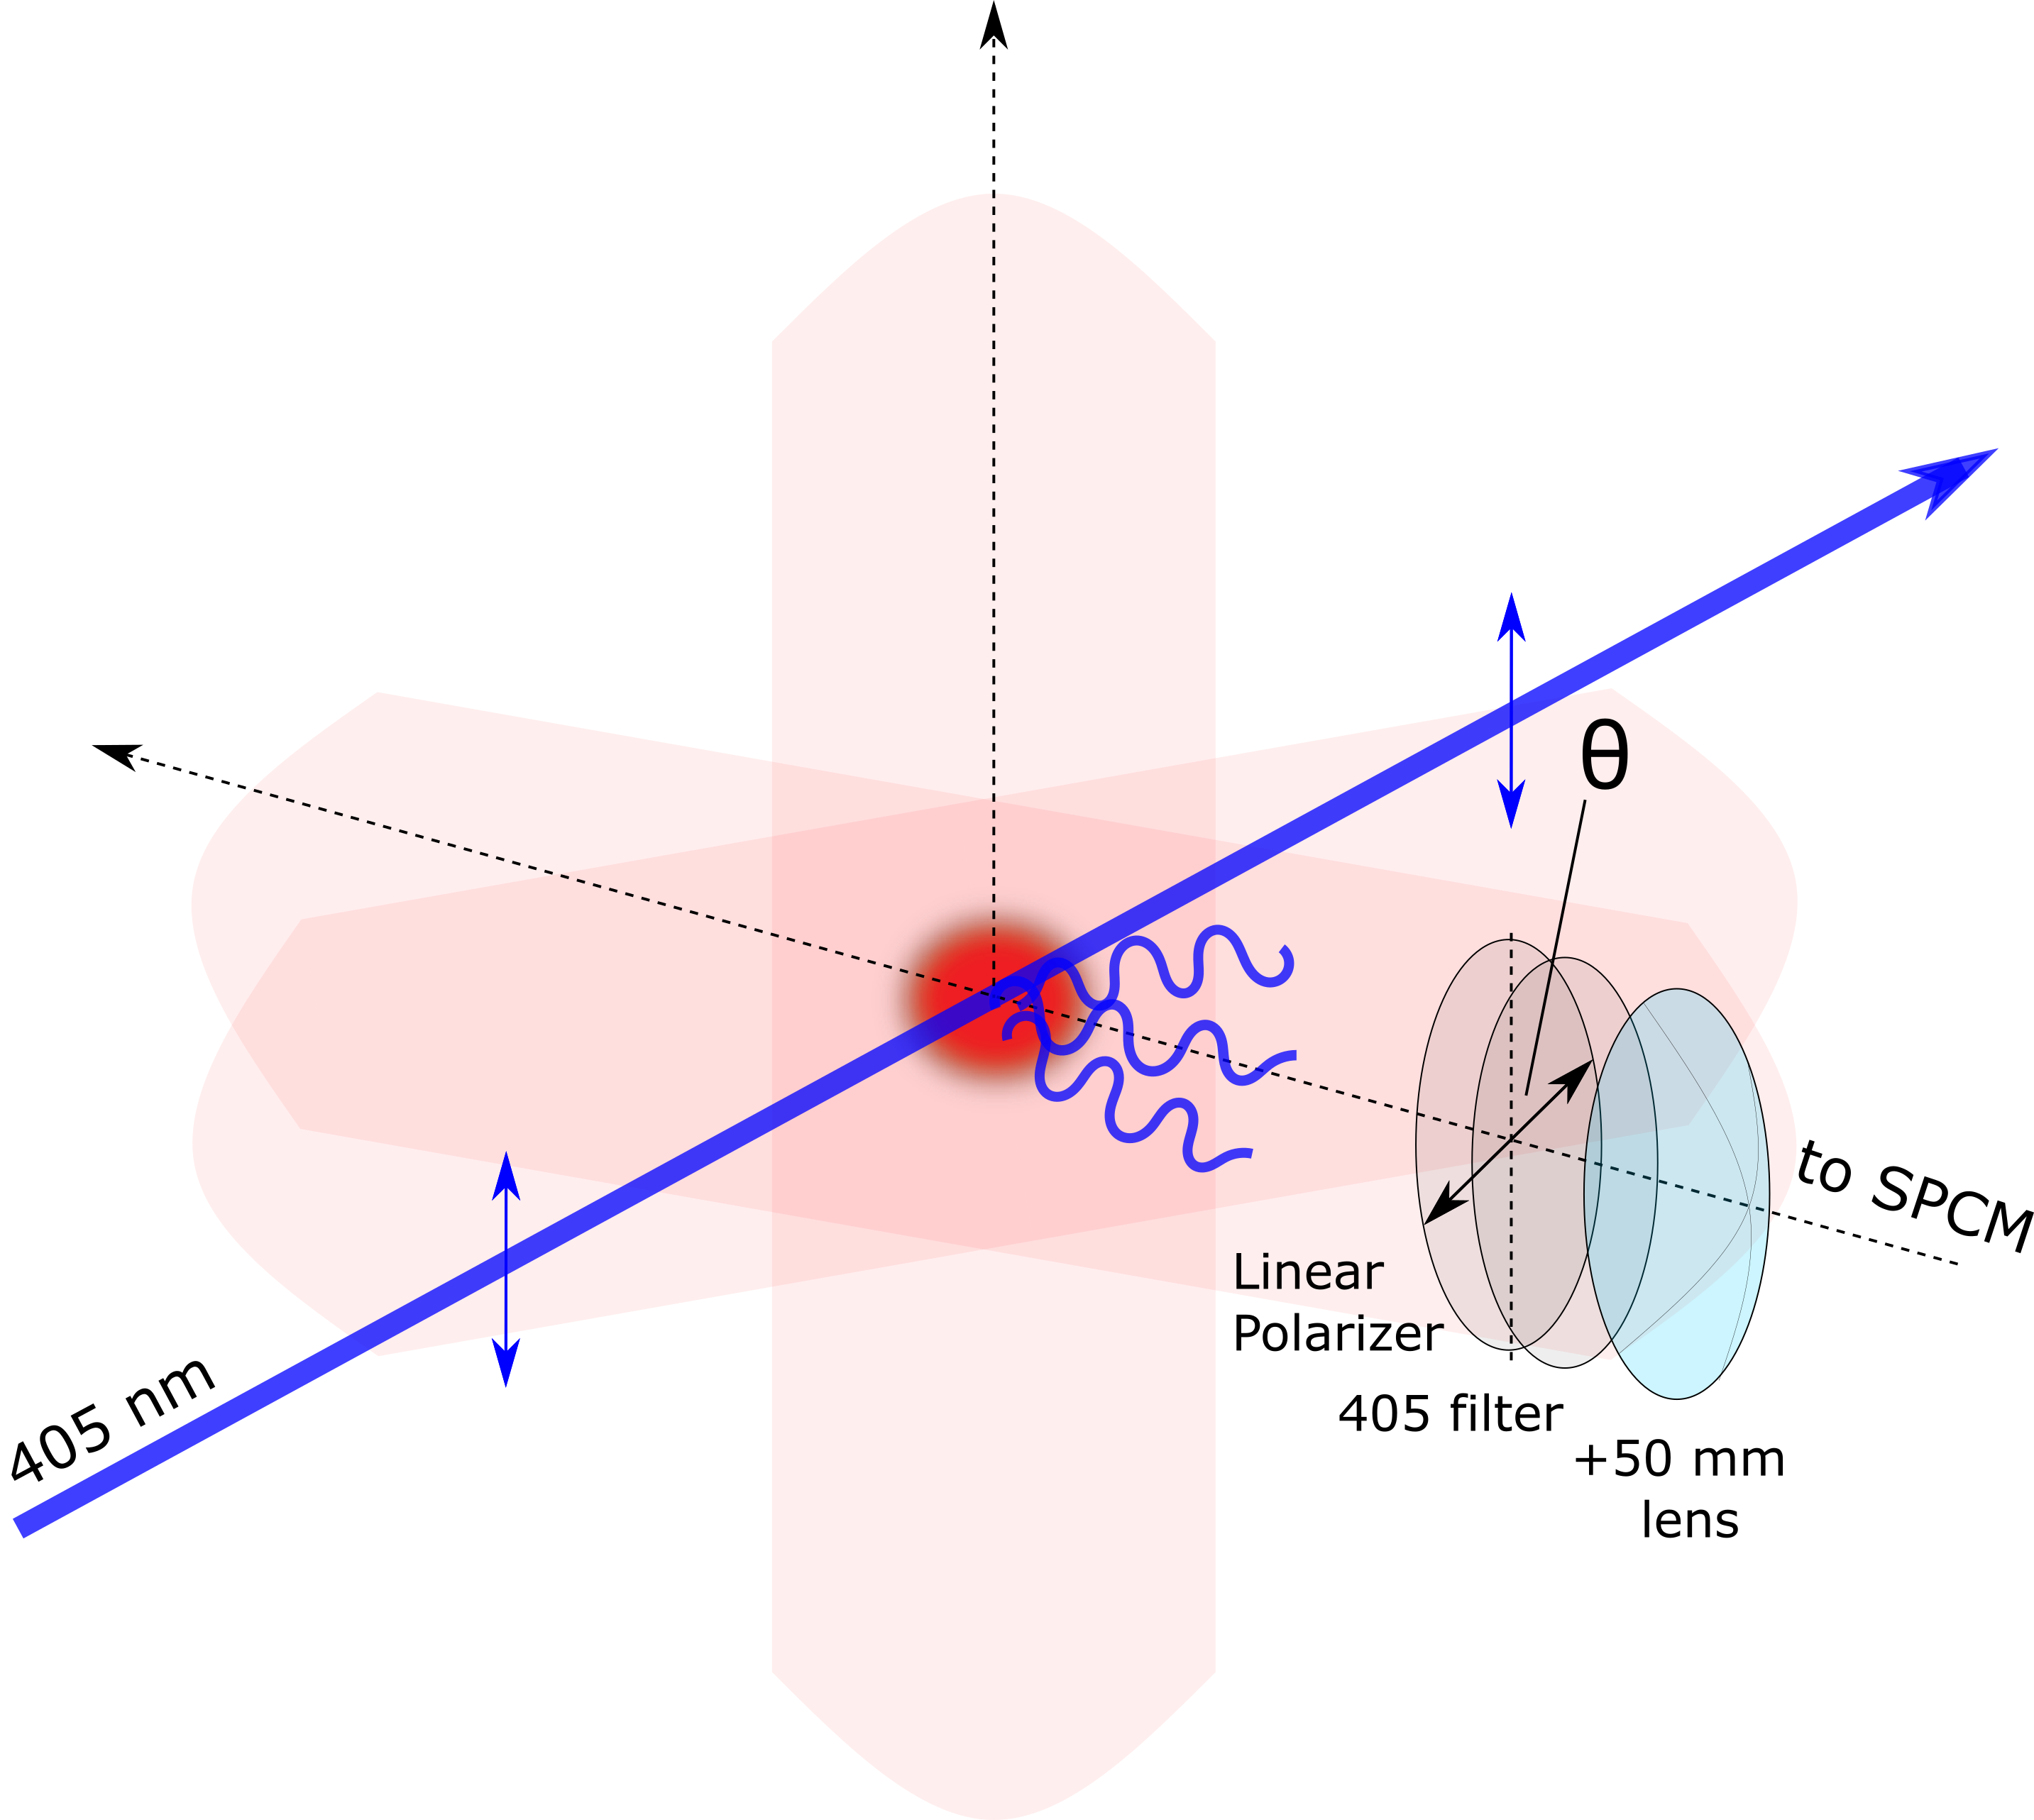
\includegraphics[width=\textwidth]{experimental_geometry}
	\end{subfigure}
	\begin{subfigure}{0.4\textwidth}
		\includegraphics[width=\textwidth]{big_beats.eps}
	\end{subfigure}
\end{figure}

\textbf{\textcolor{blue}{$\implies$ Need some understanding of the fluorescence from 5p in K-39}}

\end{frame}










\begin{frame}
\frametitle{Theory: Hyperfine Structure}


\begin{itemize}
	\item Fine structure $\sim$  Special relativity + $\mathbf{S},\mathbf{L}$ coupling (+ Darwin) 
	
	
	\begin{equation*}
	\hspace{-20 pt} \implies\text{ New quantum number: }
	\mathbf{J} = \mathbf{S} + \mathbf{L}
	\end{equation*}
	$\,$\\
	
	
	\item Hyperfine structure $\sim$ Fine structure + Nuclear spin 
	
	\begin{equation*}
	\hspace{-20 pt}\implies\text{ New quantum number: } 
	\mathbf{F} = \mathbf{J} + \mathbf{I}
	\end{equation*}
\end{itemize}

\end{frame}




\begin{frame}
\frametitle{Theory: Hyperfine Structure}


\begin{figure}[!htb]
	\centering
	\hspace{10 pt}
	\begin{subfigure}{0.49\textwidth}
		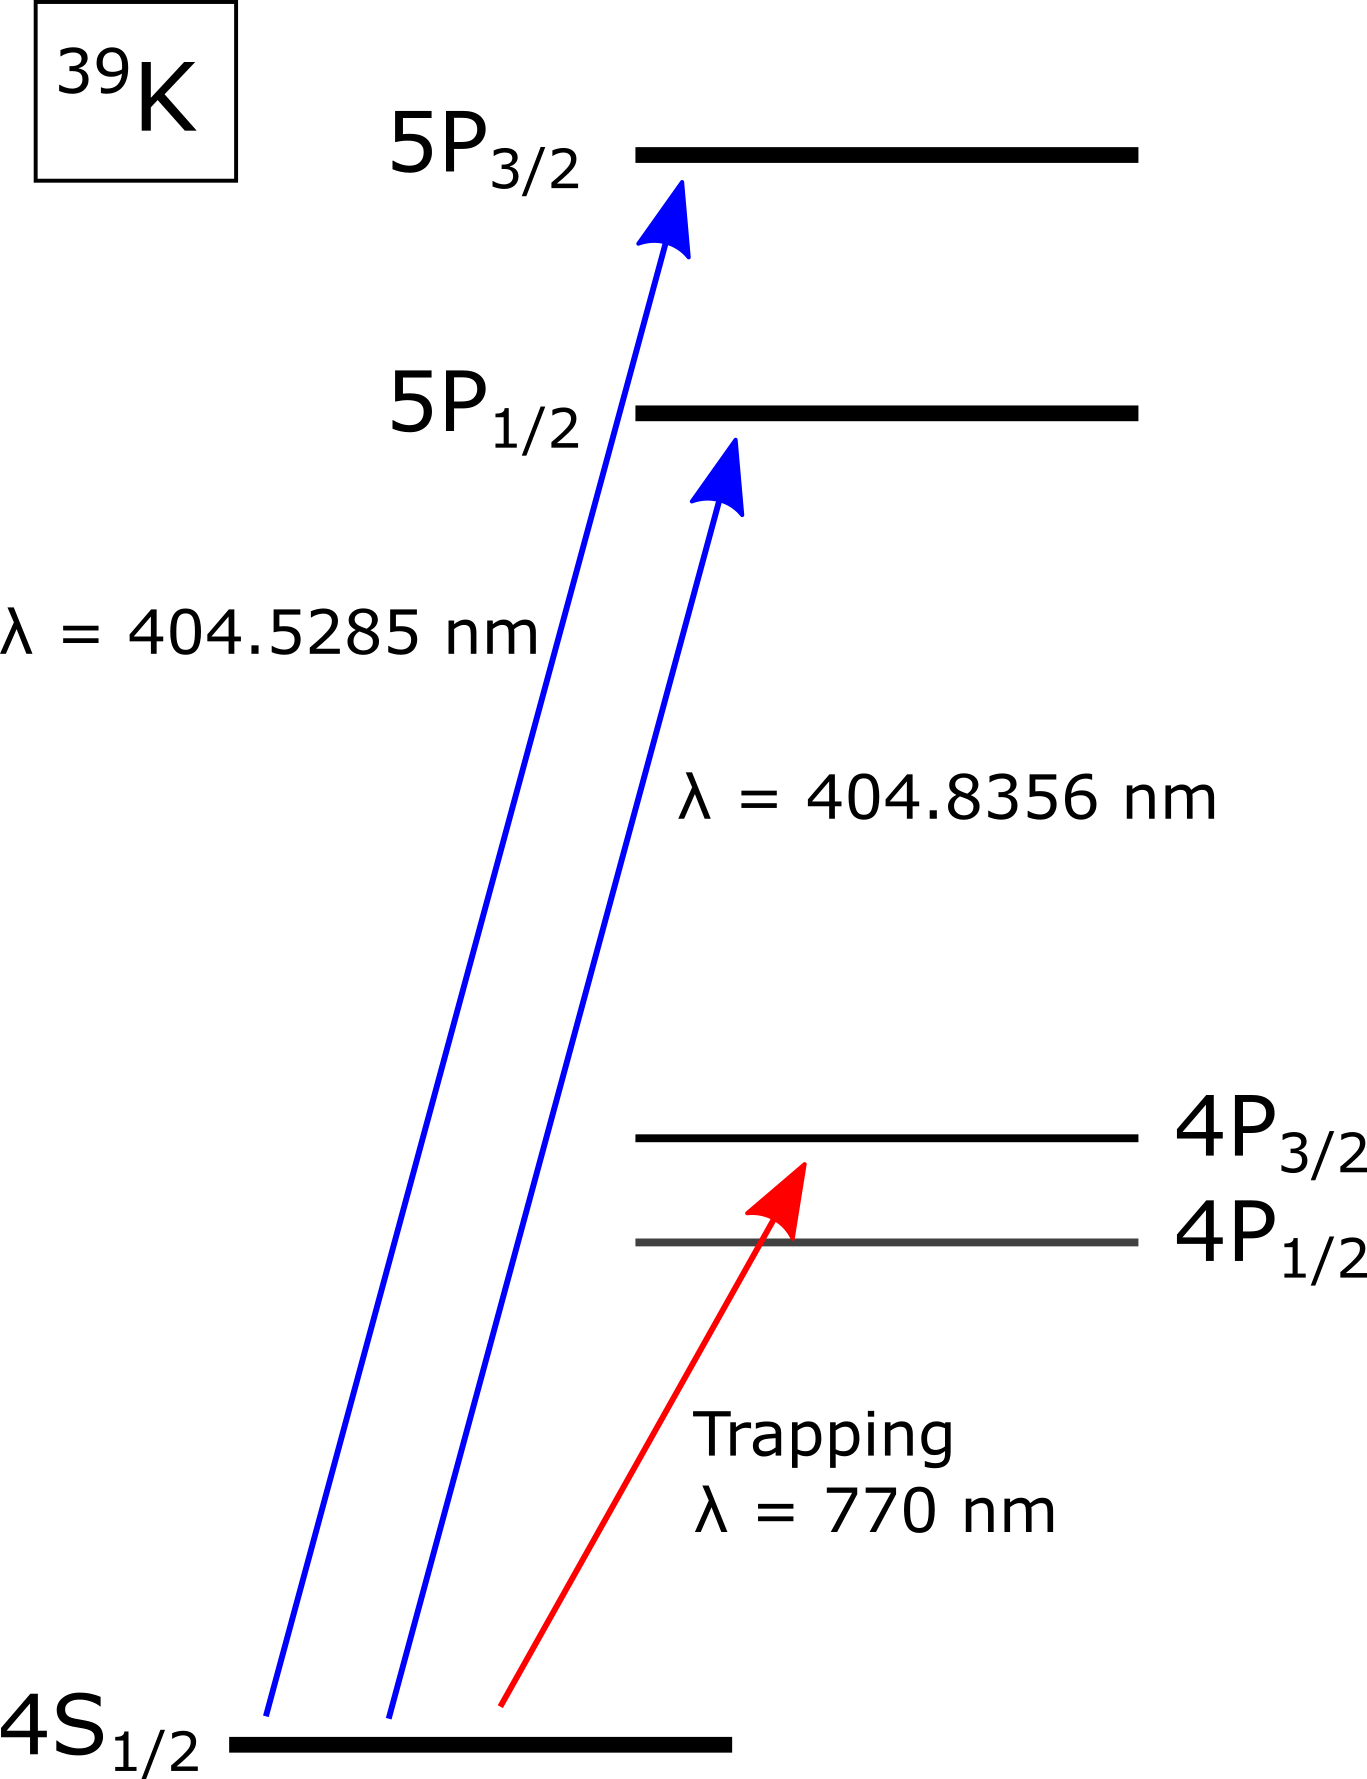
\includegraphics[width=0.8\textwidth]{energy_levels.png}
	\end{subfigure}
	\hspace{-20 pt}
	\begin{subfigure}{0.49\textwidth}
		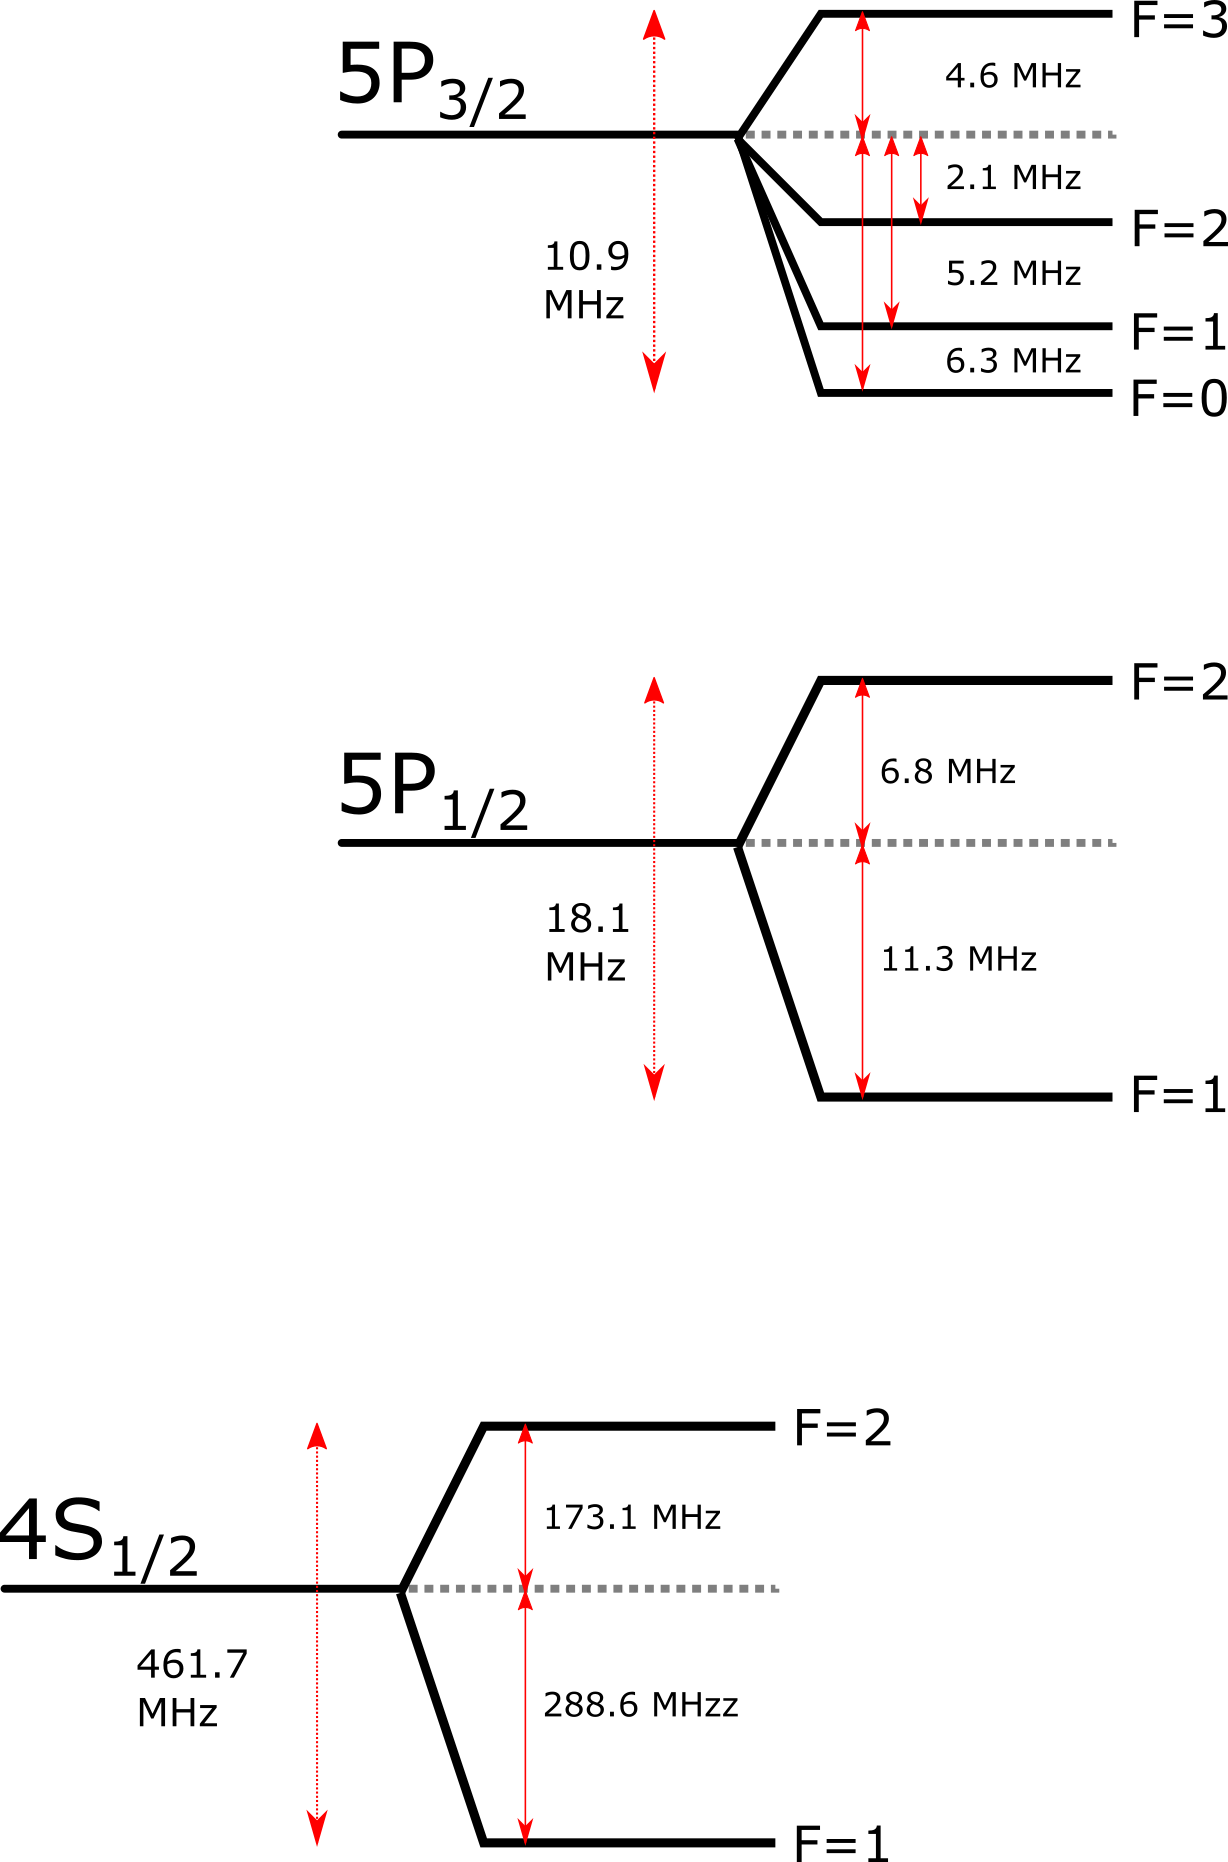
\includegraphics[width=0.7\textwidth]{hyperfine.png}
	\end{subfigure}
\end{figure}


\end{frame}














%\begin{frame}
%\frametitle{Theory: Hyperfine Structure}
%
%
%In general,
%\begin{equation*}
%\frac{1}{\tau_{fi}}= \frac{4\alpha \omega_0^3}{3c^2}\abs{ \bra{f} e \mathbf{r} \ket{i}}^2
%\end{equation*}
%
%%\begin{equation*}
%%\f{1}{\tau_{fi}} = \sum_q \f{\omega_0^3}{3\pi \epsilon_0 \hbar c^3} \abs{ \bra{f} e r_q^{(1)} \ket{i}}^2 
%%\end{equation*}
%
%
%
%For fine-structure levels,
%\begin{equation*}
%\f{1}{\tau_{JJ'}}  = \f{\omega_0^3}{3\pi \epsilon_0 \hbar c^3} \f{\abs{ \bra{nJ} \abs{e\mathbf{r}} \ket{n'J'}  }^2}{2J + 1} = A_{JJ'}
%\end{equation*}
%
%
%
%
%For hyperfine-structure levels,
%\begin{align*}
%	A_{FF'} = (2F'+1)(2J+1) \Gj{J}{F}{I}{F'}{J'}{1}^2 A_{JJ'}.
%\end{align*}
%
%
%
%\textbf{\textcolor{purple}{$\implies$ Knowing $\tau_{FF'}$ is enough to deduce $\tau_{JJ'}$}}
%
%\end{frame}



%\begin{frame}
%\frametitle{Theory: Zeeman effect}
%
%
%External magnetic fields make hyperfine sublevels nondegenerate.
%
%\begin{equation*}
%H_B= \f{\mu_B g_J}{\hbar} ( \mathbf{J} +  \mathbf{I})\cdot \mathbf{B},
%\end{equation*}
%
%
%
%$\,$\\
%
%
%In the electric quadrupole approximation,
%\begin{equation*}
%H_\text{hfs} = A_{\text{hfs}}\mathbf{I}\cdot \mathbf{J} + B_\text{hfs} \f{3(\mathbf{I}\cdot \mathbf{J})^2 + \f{3}{2}\mathbf{I}\cdot \mathbf{J} - \mathbf{I}^2\cdot \mathbf{J}^2}{2I(2I-1)J(J-1)} + \f{\mu_B}{\hbar}(g_Jm_J + g_Im_I)B
%\end{equation*}	
%
%\end{frame}




\begin{frame}
\frametitle{Theory: Zeeman effect}


\begin{figure}[!htb]
	\centering
	\vspace{-10pt}
	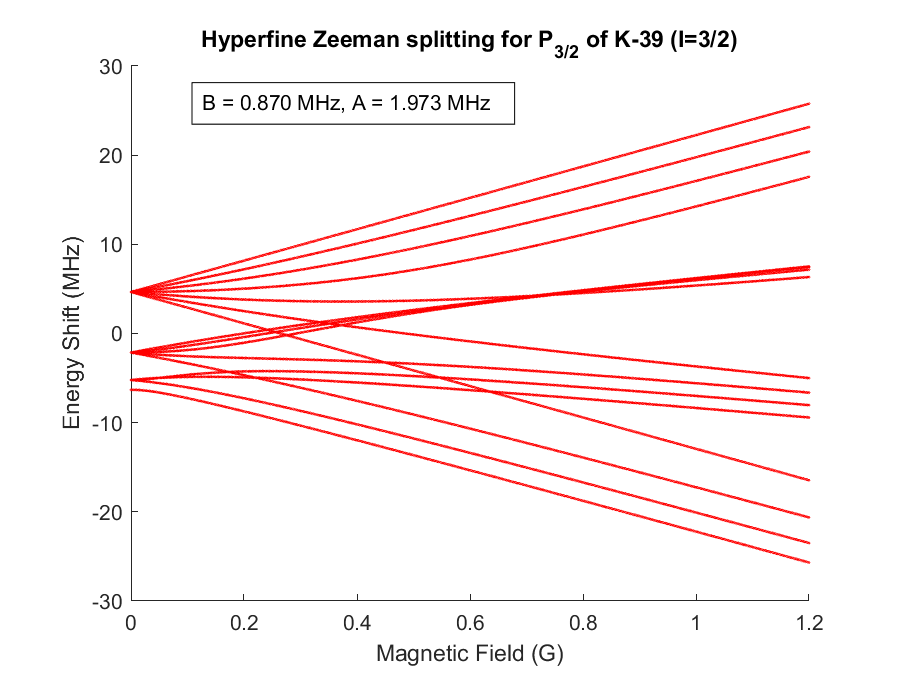
\includegraphics[height=0.7\textheight]{Zeeman_hfs.eps}
\end{figure}

\end{frame}





\begin{frame}
\frametitle{Theory: Quantum beats}

``Interference'' in fluorescence due to hyperfine sublevels 


\begin{equation*}
\ket{\psi(t)} = c_i \ket{i}e^{-i\omega_i t} + c_f \ket{f}e^{-i\omega_f t} + c_e \ket{e}e^{-i\omega_e t}
\end{equation*}



\begin{figure}[!htb]
	\centering
	\hspace{10 pt}
	\begin{subfigure}{0.49\textwidth}
		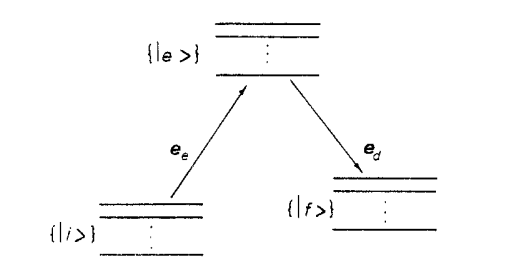
\includegraphics[width=0.85\textwidth]{energies}
	\end{subfigure}
	\hspace{-20 pt}
	\begin{subfigure}{0.49\textwidth}
		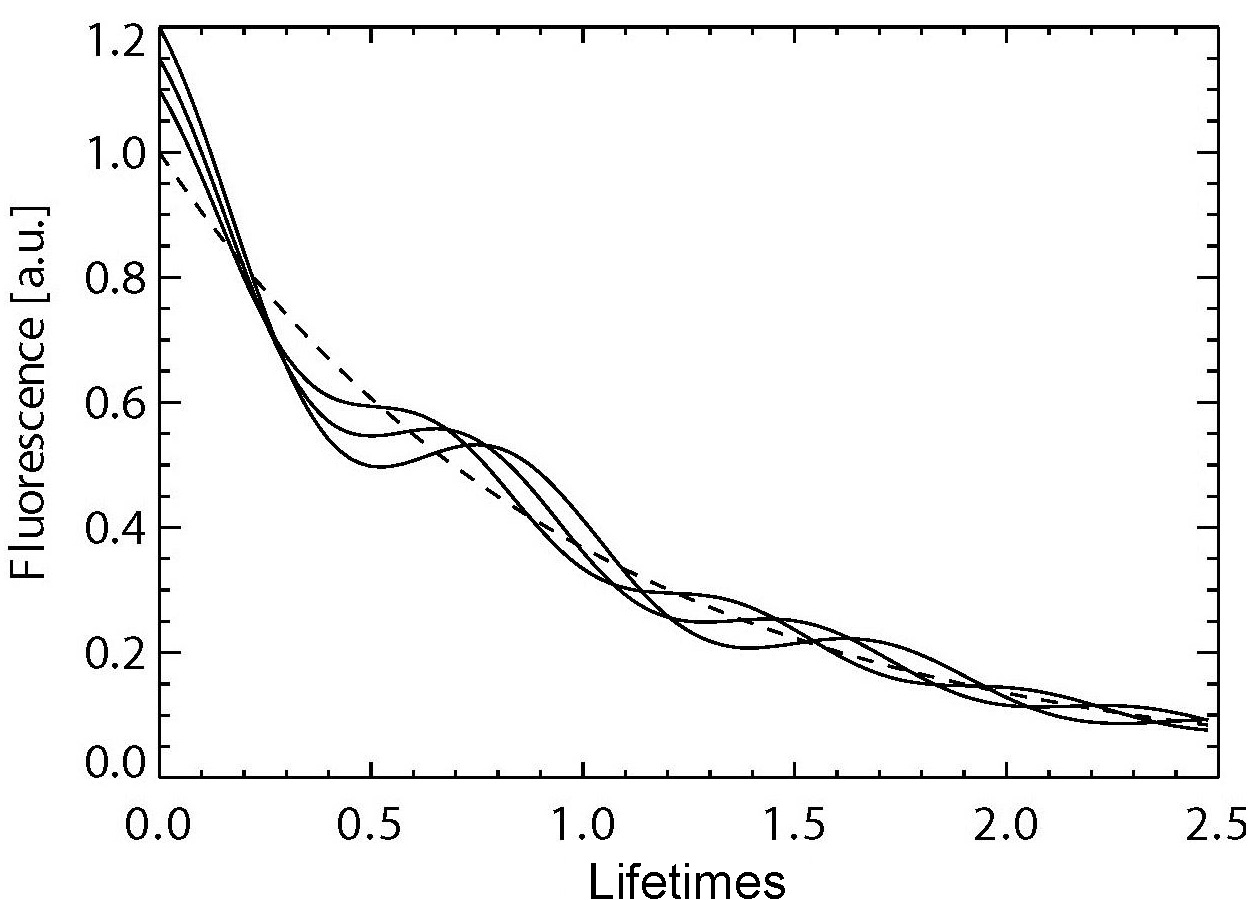
\includegraphics[width=0.65\textwidth]{qbeats1}
	\end{subfigure}
\end{figure}


The detector sees
\begin{equation*}
\abs{E}^2 = (A +  B\exp\left[i(\omega_{e} - \omega_{f})t \right] + c.c)e^{-t/\tau}.
\end{equation*}

\textbf{\textcolor{blue}{$\implies$ Difficult to extract lifetimes when quantum beats are present}}

\end{frame}




\begin{frame}
\frametitle{Theory: Quantum beats}


Quantum beats don't always occur.\\
$\,$\\


From angular momentum algebra:

\begin{itemize}
	\item Quantum beats in the $P_{1/2}$ decay: \textbf{\textcolor{olive}{NO}}\\
	
	$\implies$ $\tau_{\pOne}$ is easier to measure\\
	$\,$\\
	
	\item Quantum beats in the $P_{3/2}$ decay: \textbf{\textcolor{red}{YES}}\\
	
	$\implies$ $\tau_{\pThree}$ is difficult to measure
	
\end{itemize}


\end{frame}



\begin{frame}
\frametitle{Theory: Quantum beats}

In some cases, quantum beats can be eliminated.\\

$\implies$ The \textbf{\textcolor{purple}{magic angle}} solution: $\theta_m = \arccos(1/\sqrt{3}) \approx 54.7^\circ$

\begin{figure}[!htb]
	\centering	
	\vspace{-10pt}
	\begin{subfigure}{0.49\textwidth}
		\centering
		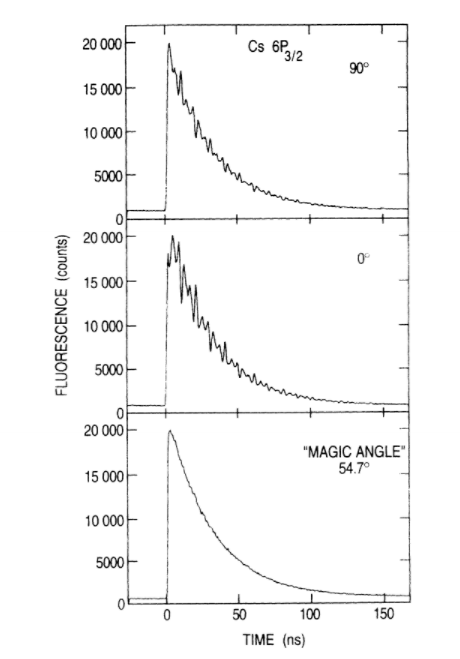
\includegraphics[width=0.7\textwidth]{young}
		\caption{Young et al. PRA 1994}
	\end{subfigure}
	\begin{subfigure}{0.49\textwidth}
		\centering
		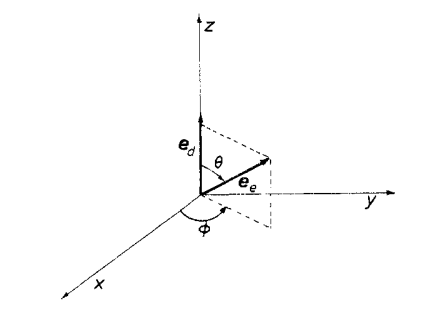
\includegraphics[width=\textwidth]{beats_1}
		\caption{$\mathbf{e}_d$: detector polarization\\
		$\hspace{17pt}\mathbf{e}_e$: excitation polarization}
	\end{subfigure}
\end{figure}



\end{frame}













\begin{frame}
\frametitle{Experiment}




\begin{figure}[!htb]
	\centering
	\hspace{10 pt}
	\begin{subfigure}{0.49\textwidth}
		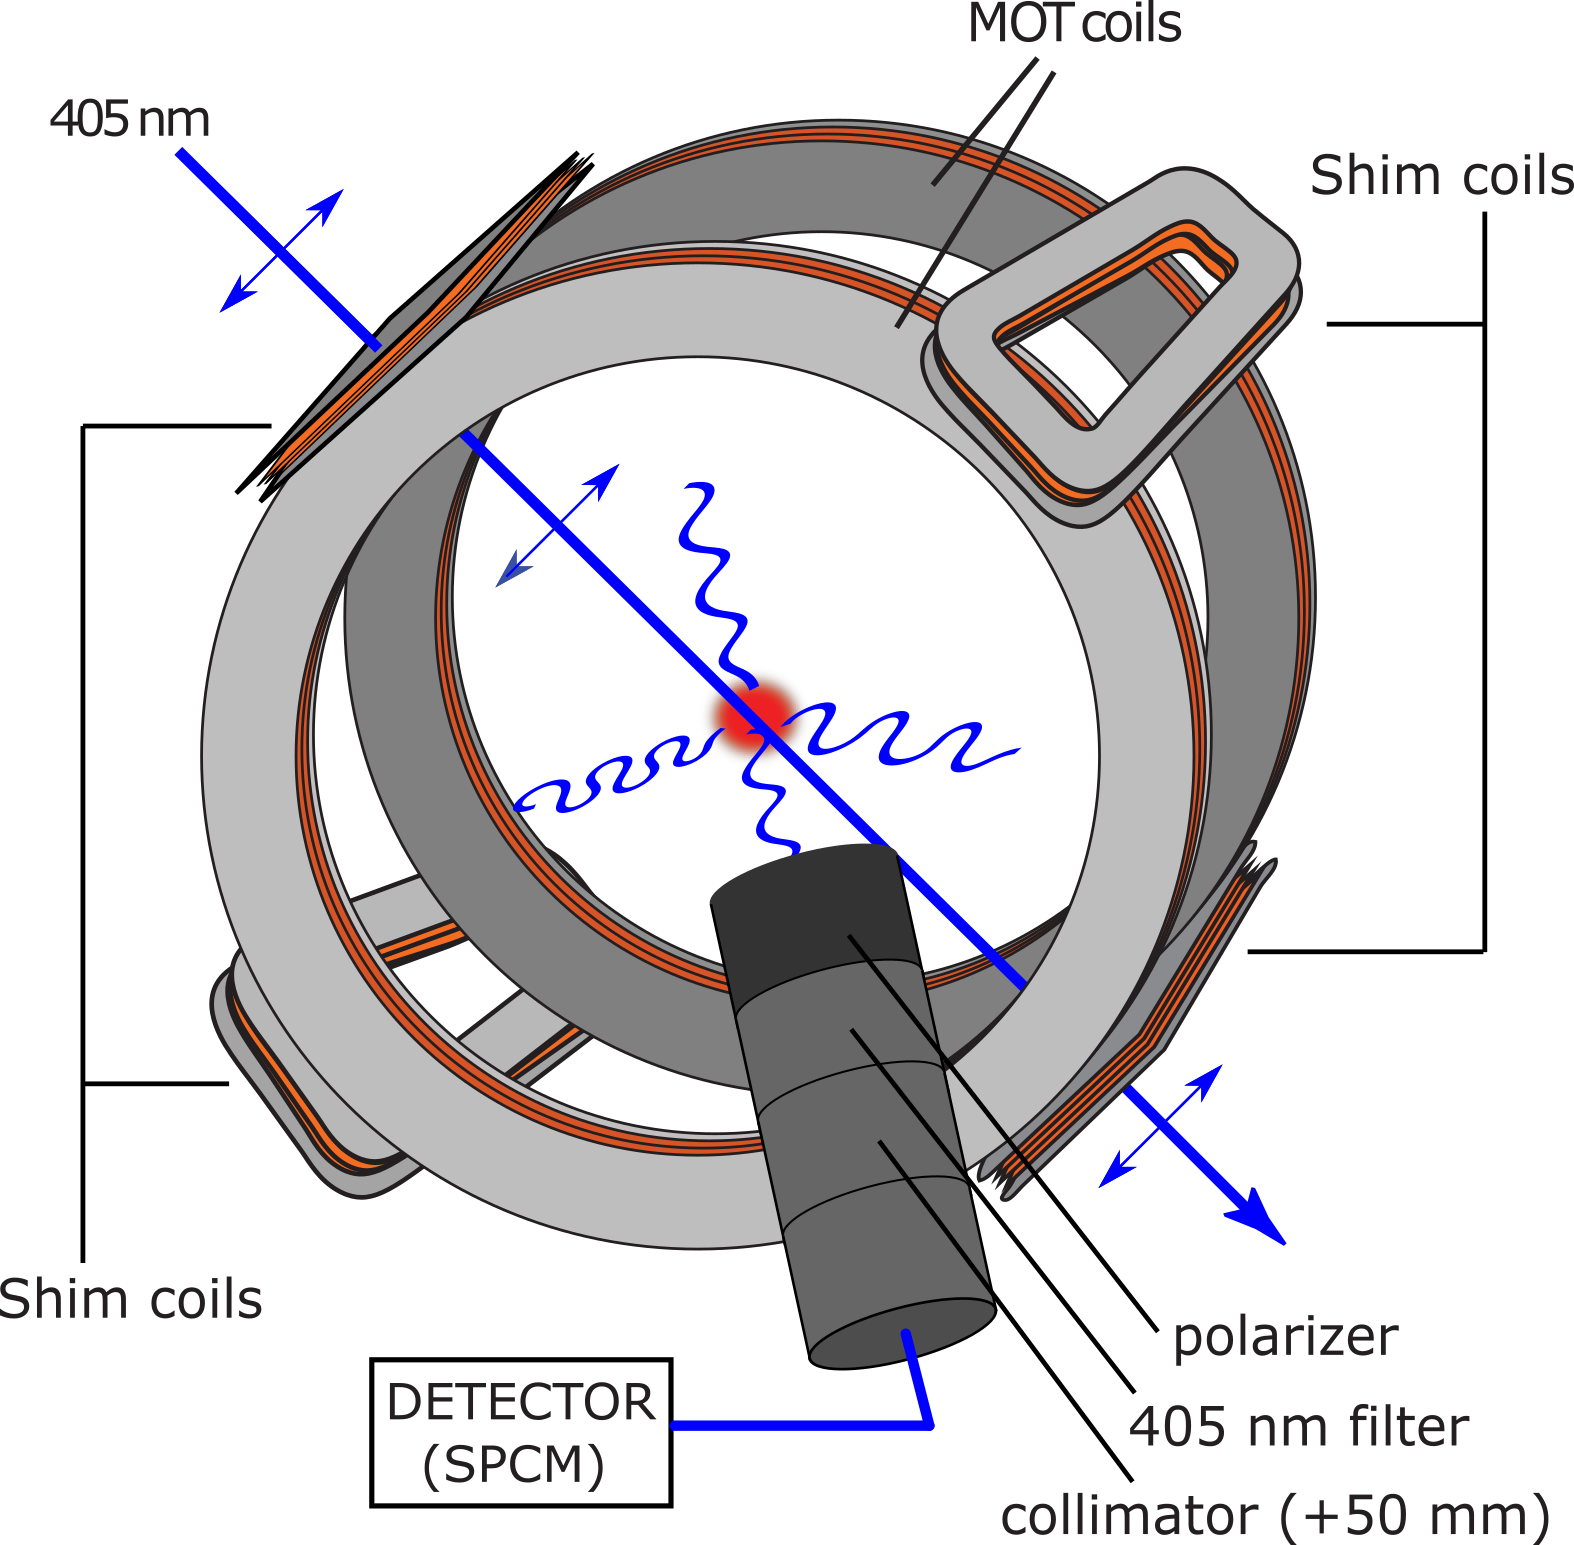
\includegraphics[width=0.9\textwidth]{MOT.png}
	\end{subfigure}
	\hspace{-20 pt}
	\begin{subfigure}{0.49\textwidth}
		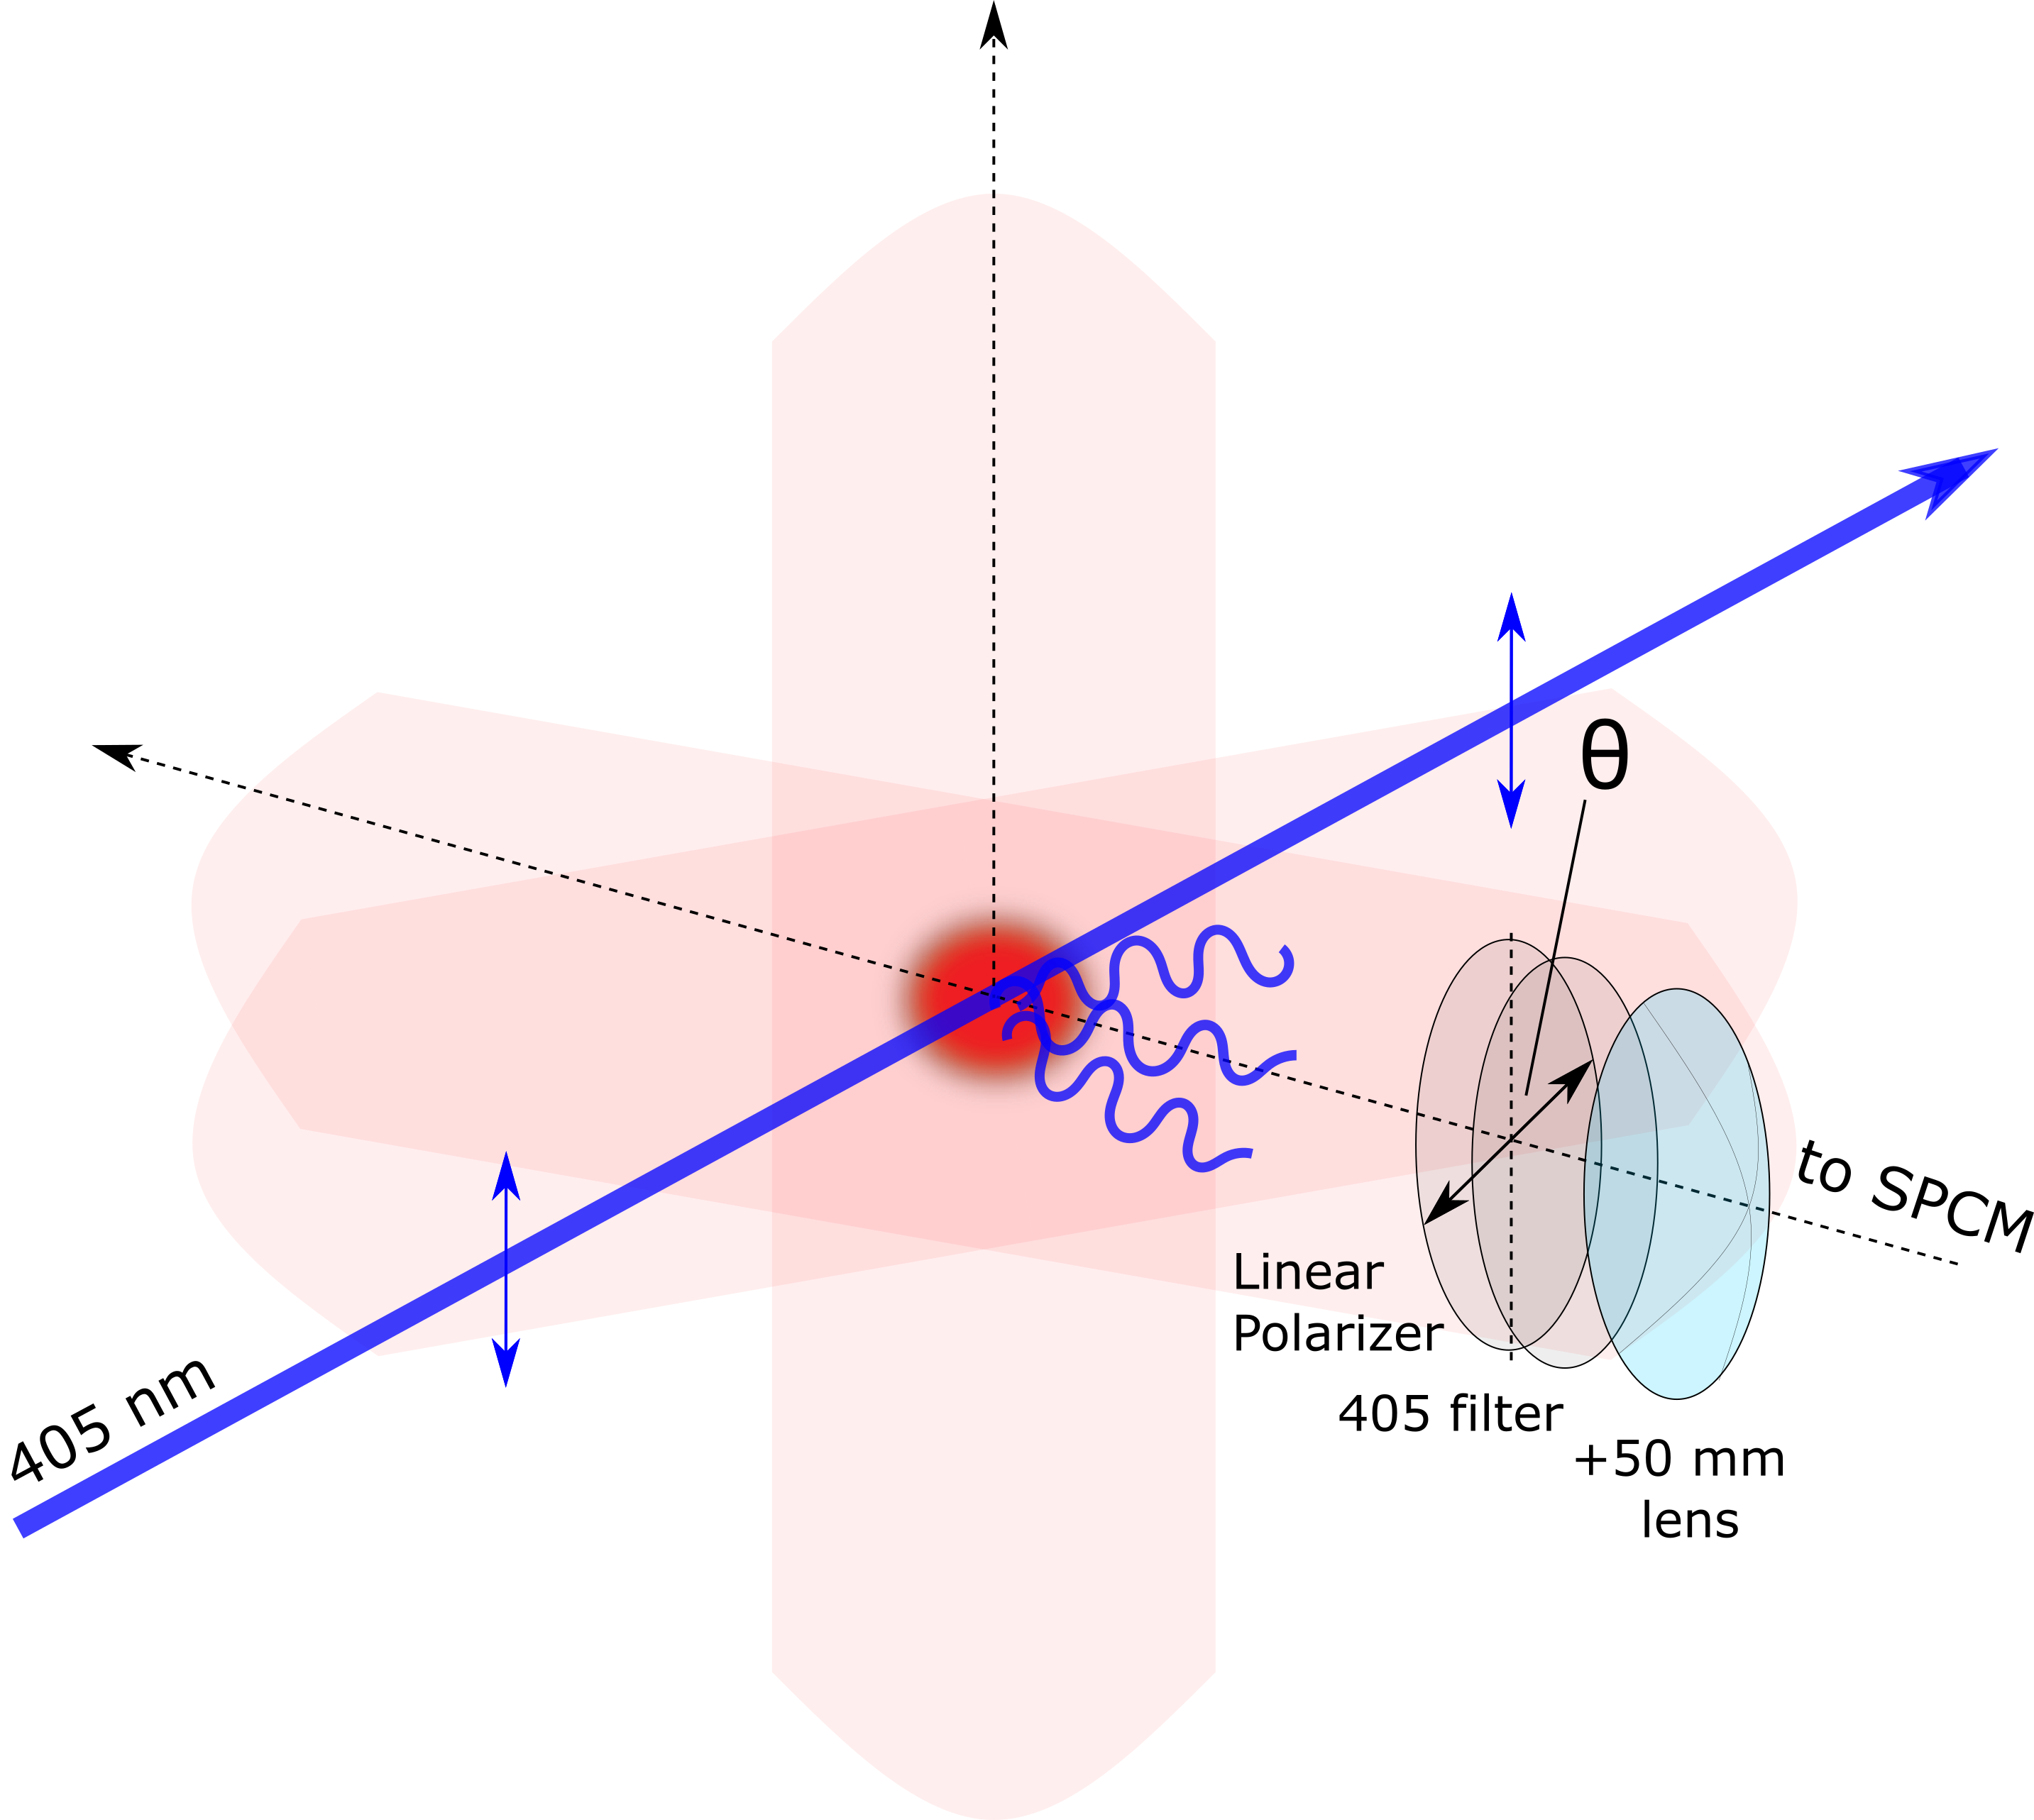
\includegraphics[width=0.9\textwidth]{experimental_geometry}
	\end{subfigure}
\end{figure}

The cloud is imaged onto an optical fiber tip. \\
The detector has QE $\sim$ 30\% at 405 nm.





\end{frame}






\begin{frame}
\frametitle{Data: 5P$_{\text{1/2}}$}


Nice, beatless, exponential decay since $J=1/2$





\begin{figure}[!htb]
	\centering
	\hspace{10 pt}
	\begin{subfigure}{0.49\textwidth}
		\includegraphics[width=\textwidth]{p12_70ns_pol.eps}
	\end{subfigure}
	\hspace{-20 pt}
	\begin{subfigure}{0.49\textwidth}
		\includegraphics[width=\textwidth]{p12_200ns_nopolar.eps}
	\end{subfigure}
\end{figure}


\end{frame}







\begin{frame}
\frametitle{Data: 5P$_{\text{1/2}}$: Error budget}


\begin{table}
	\begin{center}
		\begin{tabular}{|c|c|}
			\hline
			Source of error & Value (ns)\\ \hline
			Timing uncertainty \& Nonlinearity & $\pm$ 0.1\% \\ 
			Truncation uncertainty + pulse pile-up & $\pm$ 0.4\%\\
			Radiation trapping/rescattering & $\pm$ 0.2\% \\
			Other statistical errors &   $\pm$ 0.2\%  \\
			\hline
			Result & \textbf{138.9 $\pm$ 1.6}  \\
			\hline
			Prior result (Mills et al. (2005)) & \textbf{137.6 $\pm$ 1.3}  \\
			\hline
		\end{tabular}
	\end{center}
\end{table}
$\,$\\

$\implies$ Agreement to within $\pm \sigma.$

\end{frame}



\begin{frame}
\frametitle{Data: 5P$_{\text{1/2}}$: Radiation trapping test}



Changing the getter current changes the density of the MOT.


\begin{figure}[!htb]
	\centering
	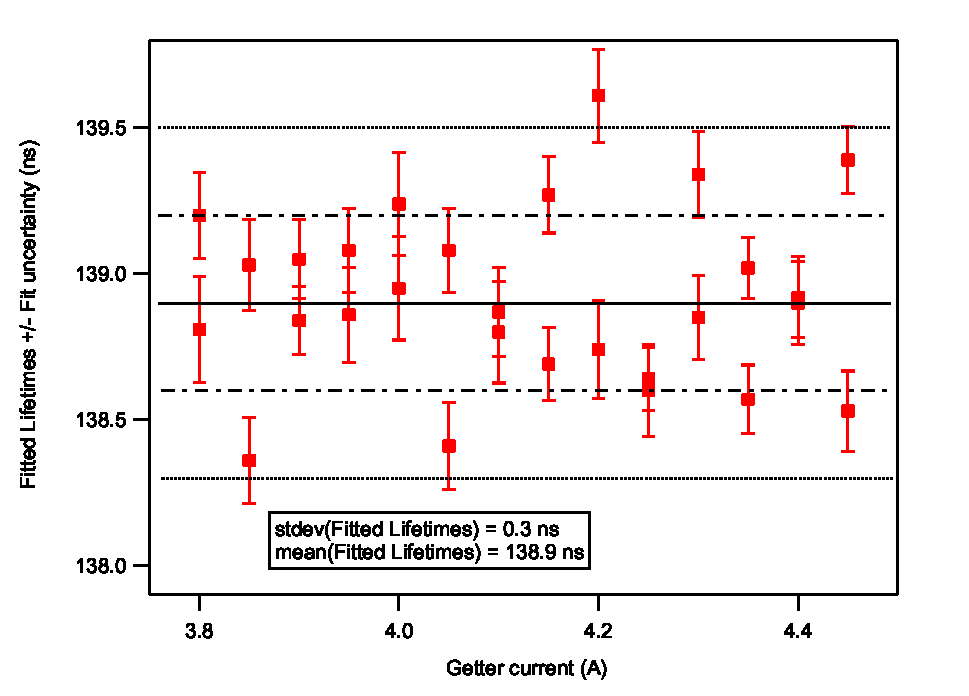
\includegraphics[width=0.7\textwidth]{getter_currents.eps}
\end{figure}



\end{frame}




\begin{frame}
\frametitle{Data: 5P$_{\text{3/2}}$}

The MOT requires a magnetic field gradient ($dB/dr \approx$ 1 G/mm) \\
$\implies$ Zeeman effects present \& vary across the cloud



\begin{figure}[!htb]
	\centering
	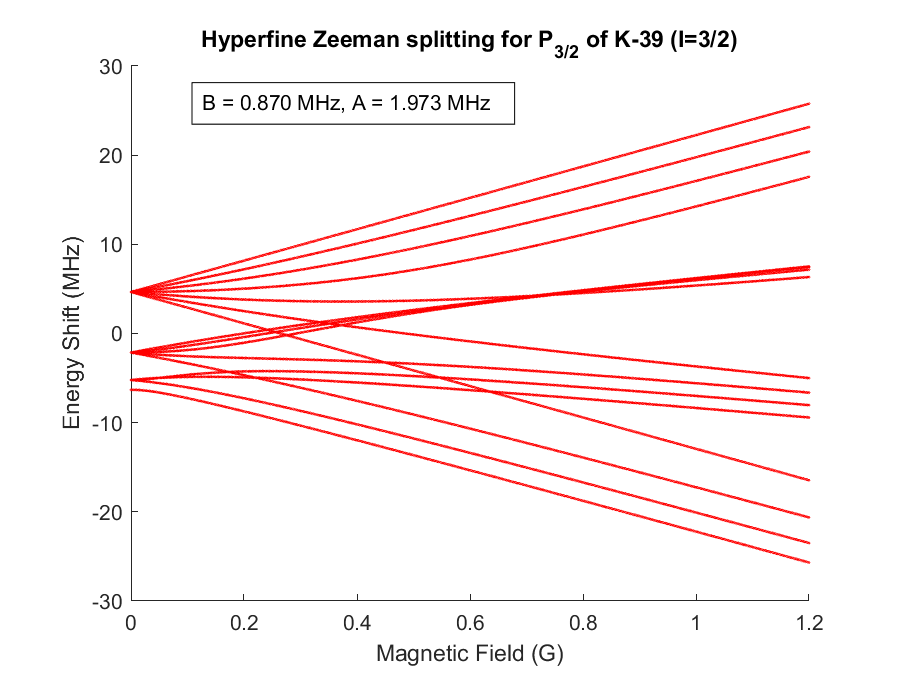
\includegraphics[height=0.7\textheight]{Zeeman_hfs.eps}
\end{figure}
\end{frame}



\begin{frame}
\frametitle{Data: 5P$_{\text{3/2}}$}

Quantum beats observed. 


\begin{figure}[!htb]
	\centering
	\includegraphics[height=0.75\textheight]{big_beats.eps}
\end{figure}


\end{frame}





\begin{frame}
\frametitle{Data: 5P$_{\text{3/2}}$}

The \textcolor{purple}{\textbf{magic angle}} trick does not eliminate beats due to Zeeman effects $\implies$ must null magnetic fields. This is easier said than done!

\begin{figure}[!htb]
	\centering
	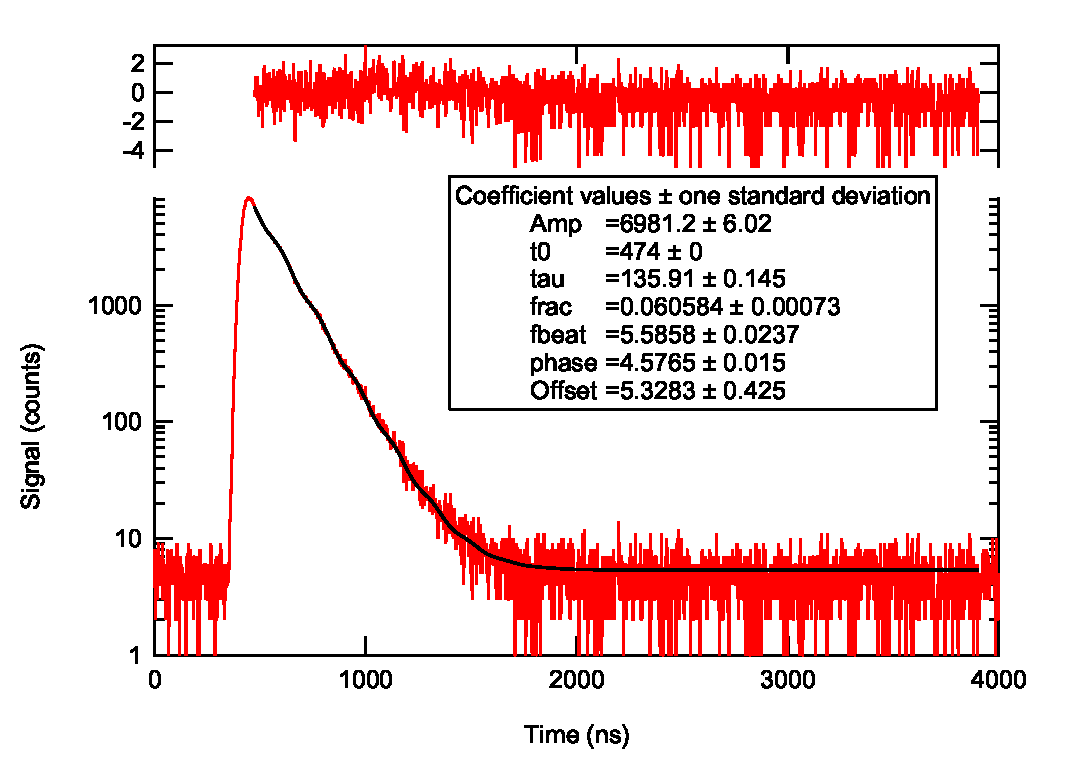
\includegraphics[width=0.75\textwidth]{small_beats_1.eps}
\end{figure}


\end{frame}



\begin{frame}
\frametitle{Data: 5P$_{\text{3/2}}$}

Exciting different parts of the MOT cloud gives different beat amplitudes.


\begin{figure}[!htb]
	\centering
	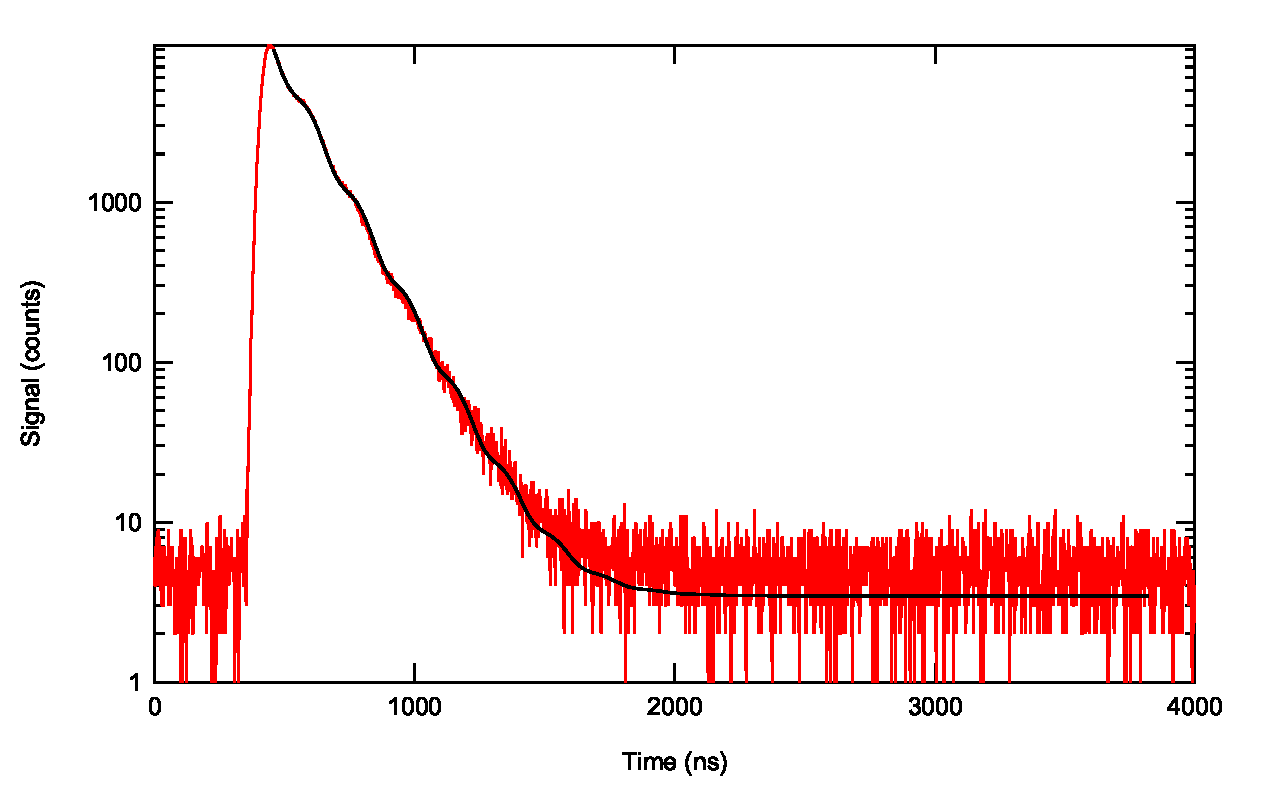
\includegraphics[width=0.75\textwidth]{big_beats_2.eps}
\end{figure}

\end{frame}






\begin{frame}
\frametitle{5P$_{\text{3/2}}$: Alternative approaches}

Using a long pulse $\implies$ removes coherence.

\begin{figure}[!htb]
	\centering
	\includegraphics[width=0.7\textwidth]{long_pulse.eps}
\end{figure}




\end{frame}




\begin{frame}
\frametitle{5P$_{\text{3/2}}$: Alternative approaches}

\begin{itemize}
	\item Hanle effect (fairly involved)
	\item Level-crossing (sweeping the magnetic field)
	\item Work with a vapor cell (many pros and cons)
	\begin{itemize}
		\item Pros: no $B$ gradient \& nulling $B$ is possible
		
		\item Cons: large Doppler width, atomic motion, large radiation trapping 
	\end{itemize}
\end{itemize}


\end{frame}


%%%%%%%%%%%%%%%%%%%%%%%%%%%%%%%%%%%%%%%%%
%%%%%%%%%%%%%%%%%%%%%%%%%%%%%%%%%%%%%%%%%
%%%%%%%%%%%%%%%%%%%%%%%%%%%%%%%%%%%%%%%%%
%%%%%%%%%%%%%%%%%%%%%%%%%%%%%%%%%%%%%%%%%
%%%%%%%%%%%%%%%%%%%%%%%%%%%%%%%%%%%%%%%%%
%%%%%%%%%%%%%%%%%%%%%%%%%%%%%%%%%%%%%%%%%



%\begin{frame}
%\frametitle{References}
%\bibliographystyle{amsalpha}
%\bibliography{references}{}
%\end{frame}



\end{document}